\chapter{Chosen-Ciphertext Attacks Security}
In this chapter we extend the security definitions of an ME to the setting of chosen-ciphertext attacks (CCA).
As in the original definition, security is defined via two properties: privacy and authenticity.

\section{Privacy}\label{sec:cca-privacy}
We want privacy to capture secrecy of the sender's inputs (i.e., the attributes $\sattr$, the policy for the receiver $\raccess$, and the plaintext $\msg$), in two different scenarios: in case of a match between the sender's and receiver's attributes/policy, and in case of mismatch.
More formally, we require that the distributions $\enc(\ek_{\sattr_0}, \raccess_0, \msg_0)$ and $\enc(\ek_{\sattr_1}, \raccess_1, \msg_1)$ are computationally indistinguishable to the eyes of an attacker with oracle access to $\skgen$, $\rkgen$, $\polgen$, where the values $(m_0, m_1,\raccess_0, \raccess_1, \sattr_0, \sattr_1)$ are all chosen by the adversary.
In order to exclude some trivial attacks, it is necessary to quantify privacy over all valid adversaries, as explained in \cite{Ateniese}.
\newline\newline
In this thesis, we aim at extending the power and the flexibility of the attacker, providing an oracle access to $\dec(\dk_\rattr, \dk_\saccess, \cipher)$, where the input is controlled by the attacker: clearly, we need to exclude the trivial attack of exploiting the oracle to directly decrypt the challenge chipertext\footnote{This is standard in CCA games definitions.}.
We introduce the formal definition of CCA privacy below for ME (Definition \ref{def:me_priv}) and A-ME too (Definition \ref{def:ame_priv}).

\begin{figure}
    \begin{pchstack}[center]
        \procedure[codesize = \scriptsize, bodylinesep=-7pt, colsep=-10cm]{\scriptsize$\NISHmatchgamecca{}_{\Pi, \adversary}(\secpar)$}{%
            (\mpk, \kpol, \msk) \getsr \setup(\secparam) \\[-2pt]
            (\msg_0, \msg_1, \raccess_0, \raccess_1, \sattr_0, \sattr_1, \aux) \getsr \adversary^{\ora_1, \ora_2, \ora_3, \ora_4}_1(\secparam, \mpk) \\[-2pt]
            b \getsr \bin \\[-2pt]
            \ek_{\sattr_b} \getsr \skgen(\msk, \sattr_b) \\[-2pt]
            \cipher \getsr \enc(\ek_{\sattr_b}, \raccess_b, \msg_b) \\[-2pt]
            b' \getsr \adversary^{\ora_1, \ora_2, \ora_3, \ora_4}_2(\secparam, \cipher, \aux) \\[-2pt]
            \text{If } (b' = b) \quad \pcreturn 1 \\[-2pt]
            \text{Else } \pcreturn 0
        }
        \pchspace
        \procedure[codesize = \scriptsize, bodylinesep=-7pt]{\scriptsize$\NISHeufgamecca{}_{\Pi, \adversary}(\secpar)$}{%
            (\mpk, \kpol, \msk) \getsr \setup(\secparam) \\[-2pt]
            (\cipher, \rattr, \saccess) \getsr \adversary^{\ora_1, \ora_2, \ora_3, \ora_5}(\secparam, \mpk) \\[-2pt]
            \dk_\rattr \getsr \rkgen(\msk, \rattr) \\[-2pt]
            \dk_{\saccess} \getsr \polgen(\kpol, \saccess) \\[-2pt]
            \msg = \dec(\dk_\rattr, \dk_{\saccess}, \cipher) \\[-2pt]
            \text{If } (\cipher \notin \mathcal{O}_{\ora_5}) \land \forall \sattr \in \cQuery_{\ora_1}:(\saccess(\sattr)=0) \land (\msg \neq \bot) \\[-2pt]
            \quad \pcreturn 1 \\[-2pt]
            \text{Else } \pcreturn 0
        }
    \end{pchstack}
    \caption{Games defining privacy and authenticity of ME. Oracles $\ora_1$, $\ora_2$, $\ora_3$ are implemented by $\skgen(\msk,\cdot)$, $\rkgen(\msk,\cdot)$, $\polgen(\kpol, \cdot)$; $\ora_4$ takes in input a tuple $(\rattr, \saccess, \cipher)$ and returns $\dec(\dk_\rattr, \dk_{\saccess}, \cipher); \ora_5$ takes in input a tuple $(\sattr, \raccess, \msg)$ and returns $\enc(\ek_\sattr, \raccess, \msg)$.}
    \label{fig:MIS-MATCH-AUTH-games-ME}
\end{figure}

\begin{definition}[Privacy of ME]\label{def:me_priv}
    We say that an ME $\Pi$ satisfies {\em privacy} if for all valid PPT adversaries $\adversary$:
    \[
        \left\lvert \Prob{\NISHmatchgamecca{}_{\Pi, \adversary}(\secpar) = 1} - \frac{1}{2} \right\rvert \leq \negl,
    \]
    where game $\NISHmatchgamecca{}_{\Pi, \adversary}(\secpar)$ is depicted in Fig.\ref{fig:MIS-MATCH-AUTH-games-ME}.
    Adversary $\adversary$ is called valid if $\forall (\rattr_i, \saccess_i, \cipher_i) \in \cQuery_{\ora_4}, \cipher_i \ne \cipher$ and $\forall \rattr \in \cQuery_{\ora_2}, \forall \saccess \in \cQuery_{\ora_3}$ it satisfies the following invariant:
    \begin{itemize}
        \item \textbf{(Mismatch condition).} Either
              \begin{align}
                   & (\raccess_0(\rattr) = \raccess_1(\rattr)=0) \lor (\saccess(\sattr_0) = \saccess(\sattr_1)=0) \nonumber                         \\
                   & \qquad \lor (\raccess_0(\rattr) = \saccess(\sattr_1)=0) \lor (\raccess_1(\rattr) = \saccess(\sattr_0)=0); \label{eq:valid_adv}
              \end{align}
        \item \textbf{(Match condition).} Or (if $\exists\hat\rattr \in \cQuery_{\ora_2}, \hat\saccess \in \cQuery_{\ora_3}$ s.t.\ Eq.~\eqref{eq:valid_adv} does not hold)
              \[
                  (\msg_0 = \msg_1) \land (\raccess_0(\rattr) =\raccess_1(\rattr)) \land (\saccess(\sattr_0) = \saccess(\sattr_1)).
              \]
    \end{itemize}
\end{definition}
\begin{figure*}
    \begin{pchstack}[center]
        \procedure[codesize = \scriptsize, bodylinesep=-7pt]{\scriptsize$\NISHmatchgamecca{\arranged}_{\Pi, \adversary}(\secpar)$}{%
            (\mpk, \msk) \getsr \setup(\secparam) \\[-2pt]
            (\msg_0, \msg_1, \raccess_0, \raccess_1, \sattr_0, \sattr_1, \aux) \getsr \adversary^{\ora_1,\ora_2, \ora_3}_1(\secparam, \mpk) \\[-2pt]
            b \getsr \bin \\[-2pt]
            \ek_{\sattr_b} \getsr \skgen(\mpk, \msk, \sattr_b) \\[-2pt]
            \cipher \getsr \enc(\mpk, \ek_{\sattr_b}, \raccess_b, \msg_b) \\[-2pt]
            b' \getsr \adversary^{\ora_1,\ora_2, \ora_3}_2(\secparam, \cipher, \aux) \\[-2pt]
            \text{If } (b' = b) \quad \pcreturn 1 \\[-2pt]
            \text{Else } \pcreturn 0
        }
        \pchspace
        \procedure[codesize = \scriptsize, bodylinesep=-7pt]{\scriptsize$\NISHeufgamecca{\arranged}_{\Pi, \adversary}(\secpar)$}{%
            (\mpk, \msk) \getsr \setup(\secparam) \\[-2pt]
            (\cipher, \rattr, \saccess) \getsr \adversary^{\ora_1,\ora_2, \ora_4}(\secparam, \mpk) \\[-2pt]
            \dk_{\rattr,\saccess} \getsr \rkgen(\mpk, \msk, \rattr, \saccess) \\[-2pt]
            \msg = \dec(\mpk, \dk_{\rattr,\saccess}, \cipher) \\[-2pt]
            \text{If } (\cipher \notin \mathcal{O}_{\ora_4(\cdot,\cdot,\cdot)}) \land \forall \sattr \in \cQuery_{\ora_1}:(\saccess(\sattr)=0) \land (\msg \neq \bot) \\[-2pt]
            \quad \pcreturn 1 \\[-2pt]
            \text{Else } \pcreturn 0
        }
    \end{pchstack}
    \caption{Games defining privacy and authenticity of A-ME. Oracles $\ora_1$, $\ora_2$ are implemented by $\skgen(\msk, \cdot)$ and $\rkgen(\msk, \cdot); \ora_3$ takes in input a tuple $(\rattr, \saccess, \cipher)$ and returns $\dec(\dk_{\rattr, \saccess}, \cipher); \ora_4$ takes in input a tuple $(\sattr, \raccess, \msg)$ and returns $\enc(\ek_\sattr, \raccess, \msg)$. }
    \label{fig:games-A-ME}
\end{figure*}

\begin{definition}[Privacy of A-ME]\label{def:ame_priv}
    An A-ME $\Pi$ satisfies {\em privacy} if for all valid PPT adversaries $\adversary$:
    \[
        \left\lvert \Prob{\NISHmatchgamecca{\arranged}_{\Pi, \adversary}(\secpar) = 1} - \frac{1}{2} \right\rvert \leq \negl,
    \]
    where game $\NISHmatchgamecca{\arranged}_{\Pi, \adversary}(\secpar)$ is depicted in Fig.~\ref{fig:games-A-ME}.
    Adversary $\adversary$ is called valid if if $\forall (\rattr_i, \saccess_i, \cipher_i) \in \cQuery_{\ora_3}, \cipher_i \ne \cipher$ and $\forall (\rattr, \saccess) \in \cQuery_{\ora_2}$ it satisfies the following invariant:
    \begin{itemize}
        \item \textbf{(Mismatch condition).} Either
              \begin{align}
                   & (\raccess_0(\rattr) = \raccess_1(\rattr)=0) \lor (\saccess(\sattr_0) = \saccess(\sattr_1)=0) \nonumber                             \\
                   & \qquad \lor (\raccess_0(\rattr) = \saccess(\sattr_1)=0) \lor (\raccess_1(\rattr) = \saccess(\sattr_0)=0); \label{eq:valid_adv_ame}
              \end{align}
        \item \textbf{(Match condition).} Or (if $\exists(\hat\rattr, \hat\saccess) \in \cQuery_{\ora_2}$ s.t.\ Eq.~\eqref{eq:valid_adv_ame} does not hold)
              \[
                  (\msg_0 = \msg_1) \land (\raccess_0(\rattr) =\raccess_1(\rattr)) \land (\saccess(\sattr_0) = \saccess(\sattr_1)).
              \]
    \end{itemize}
\end{definition}

\section{Authenticity}\label{sec:cca-auth}
Authenticity, instead, demands that the only way to produce a valid ciphertext under sender attributes $\sattr$ is to obtain an encryption key $ek_\sattr$ from the authority, thus guaranteeing that if a ciphertext decrypts correctly, then it has been created by a sender with the proper encryption key. This captures security against malicious senders and is modeled by a game in which the attacker has oracle access to $\skgen$, $\rkgen$, and $\polgen$.
The attacker's goal is to output a tuple $(\rattr, \saccess, \cipher)$ such that $\dec(dk_\rattr, \dk_\saccess, \cipher) \not= \bot$, and none of the encryption keys $ek_\sattr$ for attributes $\sattr$ (obtained by the adversary via oracle queries) satisfies the policy $\saccess$.
\newline\newline
The adversary is now given access to an encryption oracle: given in input sender attributes $\sattr$, a policy $\raccess$ and a message $m$, the attacker can compute an honestly generated ciphertext $\cipher$, without the need to obtain an encryption key $\ek_\sattr$ from the authority.
We clearly need to avoid trivial attacks: we do not allow the attacker to return as challenge ciphertext one provided by the oracle.
We introduce the formal definition of CCA privacy below for ME (Definition \ref{def:me_auth}) and A-ME too (Definition \ref{def:ame_auth}).

\subsection{The General Setting}
\begin{definition}[Authenticity of ME]\label{def:DNISHeufsecurity}
    We say that an ME $\Pi$ satisfies {\em authenticity} if for all PPT adversaries $\adversary$:
    \[
        \Prob{\NISHeufgamecca{}_{\Pi, \adversary}(\secpar) = 1} \leq \negl,
    \]
    where game $\NISHeufgamecca{}_{\Pi, \adversary}(\secpar)$ is depicted in Fig.\ref{fig:MIS-MATCH-AUTH-games-ME}.
\end{definition}
\subsection{The Arranged Setting}
\begin{definition}[Authenticity of A-ME]\label{def:SNISHeufsecurity}
    We say that an A-ME $\Pi$ satisfies {\em authenticity} if for all PPT adversaries $\adversary$:
    \[
        \Prob{\NISHeufgame{\arranged}_{\Pi,\adversary}(\secpar) = 1} \leq \negl,
    \]
    where game $\NISHeufgamecca{\arranged}_{\Pi, \adversary}(\secpar)$ is depicted in Fig.~\ref{fig:games-A-ME}.
\end{definition}

\section{CPA to CCA Transformation}\label{sec:cca-transformation}
We are going to define:
\begin{itemize}
    \item a first black-box transformation from CPA to CCA privacy, while preserving the authenticity
    \item a second black-box transformation from CPA to CCA authenticity, while preserving privacy
\end{itemize}
~\newline
It is evident that in order to achieve CCA security, we can simply apply both of these transformations in sequence: however, for sake of convenience, we will present a more efficient one which directly achieves both CCA privacy and CCA authenticity.
Figure \ref{fig:constr} gives a visual representation of the transformations presented in this thesis, explaining how to achieve CCA.
\begin{figure}[ht]
    \centering
    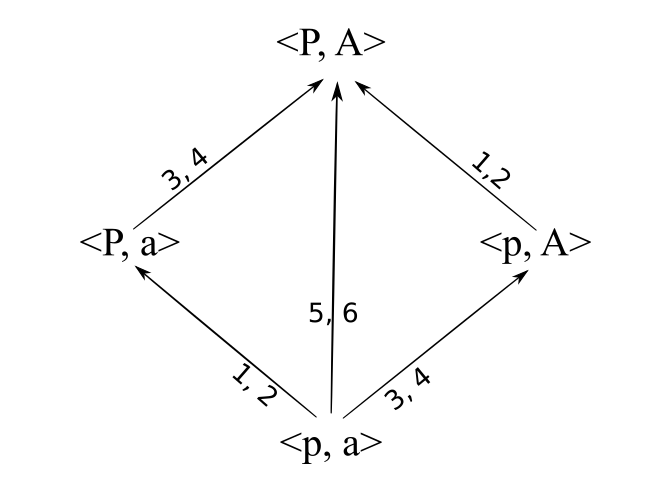
\includegraphics[width=0.7\linewidth]{images/constr.png}
    \caption{CCA Transormations Lattice. P represents Privacy, while A stands for Authenticity; the small letter indicates CPA, while the capital letter indicates CCA; the numbers refer to the corresponding theorem.}
    \label{fig:constr}
\end{figure}
\newline\newline
The starting point for our transformations are the following constructions, based on Digital Signatures and NIZK.
\begin{construction}\label{constr:me_nizk}
    Let $\Pi'=(\setup',\skgen',\rkgen', \polgen', \enc',\dec')$ be an ME scheme, $\sig =(\kgen,\sign,\ver)$ be a signature scheme $\sig$ and $\nizk=(\init,\prover,\verifier)$ be a $f$-tSE NIZK argument for the following NP relation:

    \[
        R \eqdef \Biggl\{ \begin{array}{c}((\sattr, \signature, \raccess, \msg, r),(\mpk', \pk, \cipher))\end{array}:\begin{array}{@{}c}
            \cipher = \enc'(\ek'_\sattr, \raccess, \msg; r) \land \\
            \ver(\pk, (\sattr, \signature)) = 1
        \end{array} \Biggr\}.
    \]
    \newline\newline
    We construct the new ME scheme $\Pi$ as follows:
    \begin{description}
        \item[$\setup(\secparam)$:] on input the security parameter, gets $(\msk', \kpol, \mpk') \getsr \setup'(\secparam)$, $(\sk, \pk) \getsr \kgen(\secparam)$ and $\crs \getsr \init(\secparam)$. Then outputs $\msk = (\msk', \kpol, \sk)$ as the master secret key and $\mpk = (\mpk', \pk, \crs)$ as the master public key. All other algorithms are implicitly given $\mpk$ as additional input.
        \item[$\skgen(\msk, \sattr)$:] the randomized sender-key generator takes as input the master secret key $\msk = (\msk', \sk)$ and attributes $\sattr \in \bin^*$. The algorithm returns the encryption key $\ek_\sattr = (\ek'_\sattr, \signature)$, where $\ek'_\sattr \getsr \skgen'(\msk', \sattr)$ and $\signature \getsr \sign(\sk, \sattr)$.
        \item[$\rkgen(\msk, \rattr)$:] the randomized receiver-key generator takes as input the master secret key $\msk = (\msk', \sk)$ and attributes $\rattr \in \bin^*$. The algorithm computes the key $\dk_\rattr \getsr \rkgen'(\msk', \rattr)$.
        \item[$\polgen(\kpol, \saccess)$:] the receiver policy generator takes as input the master policy key $\kpol$ and a policy $\saccess: \bin^* \to \bin$ and outputs $\dk_\saccess \getsr \polgen'(\kpol, \saccess)$.
        \item[$\enc(\ek_\sattr, \raccess, \msg)$:] the randomized encryption algorithm takes as input a secret encryption key $ek_\sattr = (\ek'_\sattr, \signature)$ for attributes $\sattr \in \bin^*$, a policy $\raccess: \bin^* \to \bin$ and a message $\msg \in \bin^*$. The algorithm first encrypts the message by computing $\cipher' \getsr \enc'(\ek'_\sattr, \raccess, \msg)$; then, it returns the ciphertext $\cipher = (\cipher', \pi)$, where $\pi \getsr \prover(\crs, (\sattr, \signature, \raccess, \msg, r),(\mpk', \pk, \cipher))$.
        \item[$\dec(\dk_\rattr, \dk_\saccess, \cipher)$:] the deterministic decryption algorithm takes as input a secret decryption key $\dk_\rattr = \dk'_\rattr$, a secret decryption key $\dk_\saccess = \dk'_\saccess$ for a circuit $\saccess: \bin^* \to \bin$ and a ciphertext $\cipher = (\cipher', \pi)$. The algorithm first checks whether $\verifier(\crs, (\cipher', \pk, \mpk'), \pi) = 0$: if true, it simply returns $\bot$; otherwise, it returns $\dec'(\dk'_\rattr, \dk_\saccess, \cipher')$.
    \end{description}
\end{construction}
Let $\Pi'$ be an A-ME scheme which satisfies privacy. If we use a signature scheme and a NIZK proof system, we can obtain a new A-ME scheme $\Pi$ which preserves its privacy, but also achieves authenticity. The construction is as follows.

\begin{construction}\label{constr:ame_nizk}
    Let $\Pi'=(\setup',\skgen',\rkgen', \enc',\dec')$ be an A-ME scheme, $\sig =(\kgen,\sign,\ver)$ be a signature scheme $\sig$ and $\nizk=(\init, \prover, \verifier)$ be a $f$-tSE NIZK argument for the following NP relation:

    \[
        R \eqdef \Biggl\{ \begin{array}{c}((\sattr, \signature, \raccess, \msg, r),(\mpk', \pk, \cipher))\end{array}:\begin{array}{@{}c}
            \cipher = \enc'(\ek'_\sattr, \raccess, \msg; r) \land \\
            \ver(\pk, (\sattr, \signature)) = 1
        \end{array} \Biggr\}.
    \]

    where $f(\sattr, \signature, \raccess, \msg, r) = (\sattr, \signature, \raccess, \msg)$, so $f$ extracts all the input but the randomness $r$.

    We construct the new A-ME scheme $\Pi$ as follows:
    \begin{description}
        \item[$\setup(\secparam)$:] on input the security parameter $\secparam$, the algorithm computes $(\msk', \mpk') \getsr \setup'(\secparam)$, $(\sk, \pk) \getsr \kgen(\secparam)$ and $\crs \getsr \init(\secparam)$. The algorithm outputs $\msk = (\msk', \sk)$ as the master secret key and $\mpk = (\mpk', \pk, \crs)$ as the master public key. All other algorithms are implicitly given $\mpk$ as additional input.
        \item[$\skgen(\msk, \sattr)$:] the randomized sender-key generator takes as input the master secret key $\msk = (\msk', \sk)$ and attributes $\sattr \in \bin^*$. The algorithm returns the encryption key $\ek_\sattr = (\ek'_\sattr, \signature)$, where $\ek'_\sattr \getsr \skgen'(\msk', \sattr)$ and $\signature \getsr \sign(\sk, \sattr)$.
        \item[$\rkgen(\msk, \rattr, \saccess)$:] the randomized receiver-key generator takes as input the master secret key $\msk = (\msk', \sk)$, attributes $\rattr \in \bin^*$ and a policy $\saccess:\bin^* \to \bin$. The algorithm computes the key $\dk_{\rattr, \saccess} \getsr \rkgen'(\msk', \rattr, \saccess)$.
        \item[$\enc(\ek_\sattr, \raccess, \msg)$:] the randomized encryption algorithm takes as input a secret encryption key $ek_\sattr = (\ek'_\sattr, \signature)$ for attributes $\sattr \in \bin^*$, a policy $\raccess: \bin^* \to \bin$ and a message $\msg \in \bin^*$. The algorithm first encrypts the message by computing $\cipher' \getsr \enc'(\ek'_\sattr, \raccess, \msg)$; then, it returns the ciphertext $\cipher = (\cipher', \pi)$, where $\pi \getsr \prover(\crs, (\sattr, \signature, \raccess, \msg, r),(\mpk', \pk, \cipher))$.
        \item[$\dec(\dk_{\rattr, \saccess}, \cipher)$:] the deterministic decryption algorithm takes as input a decryption key $\dk_{\rattr, \saccess}$ and a ciphertext $\cipher = (\cipher', \pi)$. The algorithm first checks whether $\verifier(\crs, (\cipher', \pk, \mpk'), \pi) = 0$. If true, returns $\bot$; else it returns $\dec'(\dk'_{\rattr, \saccess}, \cipher')$.
    \end{description}
\end{construction}

The correctness of the scheme follows directly by the correctness of the underlying A-ME scheme.

\begin{theorem}\label{theo:ame_nizk}
    Let $\Pi', \sig, \nizk$ be as above. If $\Pi'$ is CPA private, $\sig$ is EUF-CMA secure and $\nizk$ satisfies true-simulation extractability, then the A-ME scheme $\Pi$ from construction~\ref{constr:ame_nizk} is CCA-secure.

    \begin{proof}
        We can separately prove the two properties, by using Lemma~\ref{lemma:ame_auth} and Lemma~\ref{lemma:ame_priv}.

        \begin{lemma}\label{lemma:ame_auth}
            Construction~\ref{constr:ame_nizk} achieves CCA-authenticity.
            \begin{proof}
                The proof is almost the same as Lemma ~\ref{lemma:me_auth}: the only difference is that here we do not need to simulate anymore the generation of the policy keys.
                Let assume $\Pi$ does not achieve CCA-authenticity. This implies that there exists a valid $\adversary$ able to win with non negligible probability $\NISHeufgamecca{\arranged}_{\Pi, \adversary}(\secpar)$. If this is the case, we can build a valid $\adversary'$ to win with non negligible probability $\Sigeufgame_{\sig, \adversary'}(\secpar)$. The reduction is the following.

                \begin{enumerate}
                    \item (setup) $\adversary'$ receives the public key $\pk$ from the challenger. Then it generates the keys $(\msk', \kpol, \mpk') \getsr \setup'(\secparam)$ together with $(\crs,\tpsim,\tpext)\getsr\nizkext_0(\secparam)$. It gives $\adversary$ the master public key $\mpk = (\mpk', \pk, \crs)$.
                    \item ($\ora_1$) on input $\sattr$, $\adversary'$ invokes $\ora_\sign(\sattr)$ to receive a valid signature $\signature$ for $\sattr$. Then it runs $\ek'_\sattr \getsr \skgen'(\msk, \sattr)$ and returns $\ek_\sattr = (\ek_\sattr', \signature)$.
                    \item ($\ora_2$) on input $(\rattr, \saccess)$, $\adversary'$ returns $\ek'_{\rattr, \saccess} \getsr \rkgen'(\msk, \rattr, \saccess)$.
                    \item (encryption - $\ora_4$) on input $(\sattr, \raccess, \msg)$, computes a valid ciphertext $\cipher' \getsr \enc'(\ek'_\sattr, \raccess, \msg)$, for some $\ek'_\sattr \getsr \skgen'(\msk, \sattr)$. Then returns $\cipher = (\cipher', \pi)$, for a simulated proof $\pi = \nizksim_1(\tpsim, \cipher')$.
                    \item (challenge) on input $((\cipher', \pi), \rattr, \saccess)$, extracts $(\sattr, \signature)$, running $\nizkext_1(\tpext, \cipher', \pi)$, and forwards the tuple to the challenger.
                \end{enumerate}

                First of all, note that on setup $\adversary'$ simulates an honest challenger for $\adversary$ in all but a single event: the setup of the CRS $\crs$, indeed, is done through $\nizkext_0$, which allows $\adversary'$ to obtain the useful trapdoors. But this, clearly, does not alter (except with some negligible probability) the view of $\adversary$, because of the assumption of true-simulation extractability of $\nizk$: moreover, for the very same reason, the distribution of the proofs generated by $\ora_4$ is computationally close to the original one.
                The simulation of $\ora_2$ is tight, since it only requires keys honestly generated by $\adversary'$.
                Also $\ora_1$ queries are perfectly simulated, because of the powerful $\ora_\sign$ offered by the challenger, which allows $\adversary'$ to compute a valid signature on the sender attributes, thus preserving the correctness.

                So, by assumption, $\adversary$ wins the game with some non negligible probability, thus producing a tuple $((\cipher', \pi), \rattr, \saccess)$; in order to be acceptable, such tuple should be such that the proof is accepted and, except with some negligible probability, the extractor $\nizkext_1$ is able to reconstruct the sender attributes $\sattr$ and a valid $\signature$ on the very same attributes.
                Note that, since $\adversary$ is valid, $\adversary'$ never queries $\ora_\sign(\sattr)$: so $(\sattr, \signature)$ is a valid forgery for $\Sigeufgame_{\sig, \adversary'}(\secpar)$.
            \end{proof}
        \end{lemma}

        \begin{lemma}\label{lemma:ame_priv}
            Construction~\ref{constr:ame_nizk} achieves CCA privacy.
            \begin{proof}
                \todo{Add proof.}
                As before, this proof is almost the same as Lemma ~\ref{lemma:me_priv}: the only difference is that here we do not need to simulate anymore the generation of the policy keys.
            \end{proof}
        \end{lemma}
        Since we have shown that Construction ~\ref{constr:ame_nizk} achieves both CCA-privacy and CCA-authenticity, we have concluded the proof.
    \end{proof}
\end{theorem}
~\newline
We also give two simple variants which do not require any Signatures Scheme.
\begin{construction}\label{constr:me_nizk_priv}
    Let $\Pi'=(\setup',\skgen',\rkgen', \polgen', \enc',\dec')$ be an ME scheme, and $\nizk=(\init,\prover,\verifier)$ be a $f$-tSE NIZK argument for the following NP relation:

    \[
        R \eqdef \Biggl\{ \begin{array}{c}((\sattr, \raccess, \msg, r),(\mpk',\cipher))\end{array}:\begin{array}{@{}c}
            \cipher = \enc'(\ek'_\sattr, \raccess, \msg; r)
        \end{array} \Biggr\}.
    \]
    \newline\newline
    We construct the new ME scheme $\Pi$ as follows:
    \begin{description}
        \item[$\setup(\secparam)$:] on input $\secparam$, gets $(\msk', \kpol, \mpk') \getsr \setup'(\secparam)$, and $\crs \getsr \init(\secparam)$. Then outputs $\msk = (\msk', \kpol)$ as the master secret key and $\mpk = (\mpk', \crs)$ as the master public key. All other algorithms are implicitly given $\mpk$ as additional input.
        \item[$\skgen(\msk, \sattr)$:] the randomized sender-key generator takes as input the master secret key $\msk$ and attributes $\sattr \in \bin^*$. The algorithm returns the encryption key $\ek_\sattr \getsr \skgen'(\msk', \sattr)$.
        \item[$\rkgen(\msk, \rattr)$:] the randomized receiver-key generator takes as input the master secret key $\msk$ and attributes $\rattr \in \bin^*$. The algorithm computes the key $\dk_\rattr \getsr \rkgen'(\msk', \rattr)$.
        \item[$\polgen(\kpol, \saccess)$:] the receiver policy generator takes as input the master policy key $\kpol$ and a policy $\saccess: \bin^* \to \bin$ and outputs the decryption key $\dk_\saccess \getsr \polgen'(\kpol, \saccess)$.
        \item[$\enc(\ek_\sattr, \raccess, \msg)$:] the randomized encryption algorithm takes as input a secret encryption key $\ek_\sattr$ for attributes $\sattr \in \bin^*$, a policy $\raccess: \bin^* \to \bin$ and a message $\msg \in \bin^*$. The algorithm first encrypts the message by computing $\cipher' \getsr \enc'(\ek_\sattr, \raccess, \msg)$; then, it returns the ciphertext $\cipher = (\cipher', \pi)$, where $\pi \getsr \prover(\crs, (\sattr, \raccess, \msg, r),(\mpk', \cipher))$.
        \item[$\dec(\dk_\rattr, \dk_\saccess, \cipher)$:] the deterministic decryption algorithm takes as input a secret decryption key $\dk_\rattr$, a secret decryption key $\dk_\saccess$ for a circuit $\saccess: \bin^* \to \bin$ and a ciphertext $\cipher = (\cipher', \pi)$. The algorithm first checks whether $\verifier(\crs, (\cipher', \mpk'), \pi) = 0$: if true, it simply returns $\bot$; otherwise, it returns $\dec'(\dk'_\rattr, \dk_\saccess, \cipher')$.
    \end{description}
\end{construction}
\begin{construction}\label{constr:ame_nizk_priv}
    Let $\Pi'=(\setup',\skgen',\rkgen', \enc',\dec')$ be an A-ME scheme, and $\nizk=(\init, \prover, \verifier)$ be a $f$-tSE NIZK argument for the following NP relation:

    \[
        R \eqdef \Biggl\{ \begin{array}{c}((\sattr, \raccess, \msg, r),(\mpk', \cipher))\end{array}:\begin{array}{@{}c}
            \cipher = \enc'(\ek'_\sattr, \raccess, \msg; r)
        \end{array} \Biggr\}.
    \]
    ~\newline\newline
    We construct the new A-ME scheme $\Pi$ as follows:
    \begin{description}
        \item[$\setup, \skgen,\enc$:] Identical to the ones in construction \ref{constr:me_nizk_priv}.
        \item[$\rkgen(\msk, \rattr, \saccess)$:] the randomized receiver-key generator takes as input the master secret key $\msk = (\msk', \sk)$, attributes $\rattr \in \bin^*$ and a policy $\saccess:\bin^* \to \bin$. The algorithm computes $\dk_{\rattr, \saccess} \getsr \rkgen'(\msk', \rattr, \saccess)$.
        \item[$\dec(\dk_{\rattr, \saccess}, \cipher)$:] the deterministic decryption algorithm takes as input a decryption key $\dk_{\rattr, \saccess}$ and a ciphertext $\cipher = (\cipher', \pi)$. The algorithm first checks whether $\verifier(\crs, (\cipher', \mpk'), \pi) = 0$. If true, returns $\bot$; else it returns the same as $\dec'(\dk'_{\rattr, \saccess}, \cipher')$.
    \end{description}
\end{construction}
~\newline
The correctness of all the previous schemes follows directly by the correctness of the underlying ME (resp. A-ME) schemes.

\subsection{CCA privacy}\label{sec:cca-priv-transformation}
We define a black-box construction to transform any CPA-private ME scheme into a CCA-private ME scheme, using construction~\ref{constr:me_nizk}.
\begin{theorem}\label{theo:me_nizk_priv}
    Let $\Pi', \nizk$ be as above.
    If $\Pi'$ is CPA private, and $\nizk$ satisfies true-simulation extractability for $f(\sattr, \raccess, \msg, r) = (\sattr, \raccess, \msg)$, then the ME scheme $\Pi$ from construction~\ref{constr:me_nizk} is CCA-private and preserves its authenticity.
\end{theorem}

\begin{proof}
    We can separately prove the two properties, by using Lemma~\ref{lemma:me_priv} and Lemma~\ref{lemma:me_auth_same}.

    \begin{lemma}\label{lemma:me_priv}
        Constructions~\ref{constr:me_nizk} and \ref{constr:me_nizk_priv}  achieve CCA privacy if $f$ can extract the sender attributes $\sattr$, the policy $\raccess$ and the message $\msg$.
        \begin{proof}
            Without loss of generality, we give the proof for construction~\ref{constr:me_nizk} only: the other case is implied since it is a subcase.
            Let assume that $\Pi$ does not achieve CCA-privacy.
            This implies that there exists a valid $\adversary$ able to win with non-negligible probability $\NISHmatchgamecca{}_{\Pi, \adversary}(\secpar)$.
            If this is the case, we can build a valid $\adversary'$ to win with non-negligible probability $\NISHmatchgame{}_{\Pi', \adversary}(\secpar)$.
            The reduction is the following.

            \begin{enumerate}
                \item (setup) $\adversary'$ receives the master public key $\mpk'$ from the challenger. Then it computes $(\crs,\tpsim,\tpext)\getsr\nizkext_0(\secparam)$, the signatures keys $(\sk, \pk) \getsr \kgen(\secparam)$ and gives $\adversary$ the new master public key $\mpk = (\mpk', \pk, \crs)$.
                \item ($\ora_1$) on input $\sattr$, $\adversary'$ invokes $\ora_1(\sattr)$ to have back $\ek'_\sattr$; moreover, it computes $\signature \getsr \sign(\sk, \sattr)$. Then it gives $\adversary$ the new sender key $\ek_\sattr = (\ek'_\sattr, \signature)$.
                \item ($\ora_2$) on input $\rattr$, $\adversary'$ invokes $\ora_2(\rattr)$ and forwards the received $\ek'_\rattr$.
                \item ($\ora_3$) on input $\saccess$, $\adversary'$ invokes $\ora_3(\saccess)$ and simply forwards the received $\ek'_\saccess$.
                \item (decryption - $\ora_4$) on input $(\rattr, \saccess, (\cipher', \pi))$, it first parses the ciphertext and checks whether the proof $\pi$ is valid or not (in this case simply outputs $\bot$). Then, extracts $(\sattr, \raccess, \msg)$ using $\nizkext_1(\tpext,\cipher',\pi)$ and if there is a match returns $\msg$, otherwise returns $\bot$.
                \item (challenge) the input tuple is passed to the challenger that computes $\cipher'_b$; $\adversary'$ returns back $(\cipher'_b, \pi)$, where $\pi = \nizksim_1(\tpsim, \cipher'_b)$ is a simulated proof for $\cipher'_b$.
                \item (output) the bit $b'$ is given to the challenger.
            \end{enumerate}
            ~\newline
            The view offered by $\adversary'$ to $\adversary$ is computationally close to the original one: the difference, again, is due to the different mechanism to generate the CRS $\crs$, but this cannot be distinguished by $\adversary$, because of the assumption of f-tSE of $\nizk$.
            Oracles $\ora_2$ and $\ora_3$ are perfectly simulated since they are offered directly by the challenger.
            $\ora_1$ queries are again perfectly simulated because the sender key is honestly generated by the challenger and the signature is valid (and verifiable by $\adversary$).
            By assumption, $\ora_4$ queries are perfectly simulated except with some negligible probability, due to the failure of the extractor $\nizkext_1(\tpext, \cdot, \cdot)$: the correctness is still preserved because $\adversary'$ can extract all the necessary information to successfully decrypt a message if and only if a match occurs.
        \end{proof}
    \end{lemma}

    \begin{lemma}\label{lemma:me_auth_same}
        Construction~\ref{constr:me_nizk_priv} preserves its authenticity.
        \begin{proof}
            Let assume $\Pi$ does not preserve its authenticity.
            This implies that there exists a valid $\adversary$ able to win with non negligible probability $\NISHeufgame{}_{\Pi, \adversary}(\secpar)$ (resp. $\NISHeufgamecca{}_{\Pi, \adversary}(\secpar)$).
            If this is the case, we can build a valid $\adversary'$ to win with non negligible probability $\NISHeufgame{}_{\Pi', \adversary}(\secpar)$ (resp. $\NISHeufgamecca{}_{\Pi', \adversary}(\secpar)$).
            The reduction is the following.

            \begin{enumerate}
                \item (setup) $\adversary'$ receives the master public key $\mpk'$ from the challenger. Then it computes $(\crs,\tpsim,\tpext)\getsr\nizkext_0(\secparam)$, and gives $\adversary$ the new master public key $\mpk = (\mpk', \crs)$.
                \item ($\ora_1$) on input $\sattr$, $\adversary'$ invokes \item ($\ora_1$) on input $\sattr$, $\adversary'$ invokes $\ora_1(\sattr)$ to have back the sender key $\ek_\sattr$ which is forwarded to the $\adversary$.
                \item ($\ora_2$) on input $\rattr$, $\adversary'$ invokes $\ora_2(\rattr)$ and forwards the received $\ek'_\rattr$.
                \item ($\ora_3$) on input $\saccess$, $\adversary'$ invokes $\ora_3(\saccess)$ and simply forwards the received $\ek'_\saccess$.
                \item (encryption - $\ora_5$)\footnote{only for CCA game} invokes $\ora_5(\rattr)$ and forwards the received ciphertext $\cipher$.
                \item (challenge) on input $((\cipher', \pi), \rattr, \saccess)$, forwards the tuple $(\cipher, \rattr, \saccess)$ to the challenger.
            \end{enumerate}
        \end{proof}
    \end{lemma}
    ~\newline
    Since we have shown that Construction~\ref{constr:me_nizk_priv} achieves CCA-privacy and preserves its authenticity, we have concluded the proof.
\end{proof}

~\newline
In order to achieve CCA-private A-ME schemes, we can rely on construction~\ref{constr:ame_nizk} and define the following transormation.
\begin{theorem}\label{theo:ame_nizk_priv}
    Let $\Pi', \nizk$ be as above.
    If $\Pi'$ is CPA private, and $\nizk$ satisfies true-simulation extractability for $f(\sattr, \signature, \raccess, \msg, r) = (\sattr, \raccess, \msg)$, then the ME scheme $\Pi$ from construction~\ref{constr:ame_nizk_priv} is CCA-private and preserves its authenticity.
\end{theorem}

\begin{proof}
    We can separately prove the two properties, by using Lemma~\ref{lemma:ame_priv} and Lemma~\ref{lemma:ame_auth_same}

    \begin{lemma}\label{lemma:ame_priv}
        Constructions~\ref{constr:ame_nizk} and \ref{constr:ame_nizk_priv} achieve CCA privacy.
        \begin{proof}
            As before, this proof is almost the same as Lemma ~\ref{lemma:me_priv} (wlog, we only prove the lemma for construction~\ref{constr:ame_nizk}): the only difference is that here we do not need to simulate anymore the generation of the policy keys.
            Let assume that $\Pi$ does not achieve CCA-privacy.
            This implies that there exists a valid $\adversary$ able to win with non-negligible probability $\NISHmatchgamecca{\arranged}_{\Pi, \adversary}(\secpar)$.
            If this is the case, we can build a valid $\adversary'$ to win with non-negligible probability $\NISHmatchgame{\arranged}_{\Pi', \adversary'}(\secpar)$.
            The reduction is the following.

            \begin{enumerate}
                \item (setup) $\adversary'$ receives the master public key $\mpk'$ from the challenger. Then it computes $(\crs,\tpsim,\tpext)\getsr\nizkext_0(\secparam)$, the signatures keys $(\sk, \pk) \getsr \kgen(\secparam)$ and gives $\adversary$ the new master public key $\mpk = (\mpk', \pk, \crs)$.
                \item ($\ora_1$) on input $\sattr$, $\adversary'$ invokes $\ora_1(\sattr)$ to have back $\ek'_\sattr$; moreover, it computes $\signature \getsr \sign(\sk, \sattr)$. Then it gives $\adversary$ the new sender key $\ek_\sattr = (\ek'_\sattr, \signature)$.
                \item ($\ora_2$) on input $(\rattr, \saccess)$, $\adversary'$ invokes $\ora_2(\rattr, \saccess)$ and forwards the received $\dk_{\rattr, \saccess}$.
                \item (decryption - $\ora_3$) on input $(\rattr, \saccess, (\cipher', \pi))$, it first parses the ciphertext and checks whether the proof $\pi$ is valid or not (in this case simply outputs $\bot$). Then, extracts $(\sattr, \signature, \raccess, \msg)$ using $\nizkext_1(\tpext,\cipher',\pi)$ and if there is a match returns $\msg$, otherwise returns $\bot$.
                \item (challenge) the input tuple is passed to the challenger that computes $\cipher'_b$; $\adversary'$ returns back $(\cipher'_b, \pi)$, where $\pi = \nizksim_1(\tpsim, \cipher'_b)$ is a simulated proof for $\cipher'_b$.
                \item (output) the bit $b'$ is given to the challenger.
            \end{enumerate}
            ~\newline
            The view offered by $\adversary'$ to $\adversary$ is computationally close to the original one: the difference, again, is due to the different mechanism to generate the CRS $\crs$, but this cannot be distinguished by $\adversary$, because of the assumption of f-tSE of $\nizk$.
            Oracles$\ora_2$ is perfectly simulated since it is offered directly by the challenger.
            $\ora_1$ queries are again perfectly simulated because the sender key is honestly generated by the challenger and the signature is valid (and verifiable by $\adversary$).
            By assumption, $\ora_3$ queries are perfectly simulated except with some negligible probability, due to the failure of the extractor $\nizkext_1(\tpext, \cdot, \cdot)$: the correctness is still preserved because $\adversary'$ can extract all the necessary information to successfully decrypt a message if and only if a match occurs.
        \end{proof}
    \end{lemma}

    \begin{lemma}\label{lemma:ame_auth_same}
        Construction~\ref{constr:ame_nizk} preserves its authenticity.
        \begin{proof}
            Let assume $\Pi$ does not preserve its authenticity.
            This implies that there exists a valid $\adversary$ able to win with non negligible probability $\NISHeufgame{\arranged}_{\Pi, \adversary}(\secpar)$ (resp. $\NISHeufgamecca{\arranged}_{\Pi, \adversary}(\secpar)$).
            If this is the case, we can build a valid $\adversary'$ to win with non negligible probability $\NISHeufgame{\arranged}_{\Pi', \adversary'}(\secpar)$ (resp. $\NISHeufgamecca{\arranged}_{\Pi', \adversary'}(\secpar)$).
            The reduction is the following.

            \begin{enumerate}
                \item (setup) $\adversary'$ receives the master public key $\mpk'$ from the challenger. Then it computes $(\crs,\tpsim,\tpext)\getsr\nizkext_0(\secparam)$, the signatures keys $(\sk, \pk) \getsr \kgen(\secparam)$ and gives $\adversary$ the new master public key $\mpk = (\mpk', \pk, \crs)$.
                \item ($\ora_1$) on input $\sattr$, $\adversary'$ invokes \item ($\ora_1$) on input $\sattr$, $\adversary'$ invokes $\ora_1(\sattr)$ to have back $\ek'_\sattr$; moreover, it computes $\signature \getsr \sign(\sk, \sattr)$. Then it gives $\adversary$ the new sender key $\ek_\sattr = (\ek'_\sattr, \signature)$.
                \item ($\ora_2$) on input $\rattr$, $\adversary'$ invokes $\ora_2(\rattr, \saccess)$ and forwards the received $\dk_{\rattr, \saccess}$.
                \item (encryption - $\ora_4$)\footnote{Only for CCA game.} invokes $\ora_4(\rattr)$ and forwards the received ciphertext $\cipher$.
                \item (challenge) on input $((\cipher', \pi), \rattr, \saccess)$, forwards the tuple $(\cipher, \rattr, \saccess)$ to the challenger.
            \end{enumerate}
        \end{proof}
    \end{lemma}
    ~\newline
    Since we have shown that Construction~\ref{constr:ame_nizk_priv} achieves CCA-privacy and preserves its authenticity, we have concluded the proof.
\end{proof}


\subsection{CCA authenticity}\label{sec:cca-auth-transformation}
We define a black-box construction to achieve CCA-authenticity, using construction~\ref{constr:me_nizk}.
\begin{theorem}\label{theo:me_nizk_auth}
    Let $\Pi', \sig, \nizk$ be as above.
    If $\Pi'$ has CPA authenticity, $\sig$ is EUF-CMA secure and $\nizk$ satisfies true-simulation extractability for $f$ such that $f(\sattr, \signature, \raccess, \msg, r) = (\sattr, \raccess, \msg)$, then the ME scheme $\Pi$ from construction~\ref{constr:me_nizk} achieves CCA authenticity and preserves its privacy.
\end{theorem}

\begin{proof}
    We can separately prove the two properties, by using Lemma~\ref{lemma:me_priv_same} and Lemma~\ref{lemma:me_auth}

    \begin{lemma}\label{lemma:me_priv_same}
        Construction~\ref{constr:me_nizk} preserves CPA (resp. CCA) privacy.
        \begin{proof}
            Let assume that $\Pi$ does not preserve its privacy.
            This implies that there exists a valid $\adversary$ able to win with non negligible probability $\NISHmatchgame{}_{\Pi, \adversary}(\secpar)$ (resp. $\NISHmatchgamecca{}_{\Pi, \adversary}(\secpar)$).
            If this is the case, we can build a valid $\adversary'$ to win with non negligible probability $\NISHmatchgame{}_{\Pi', \adversary'}(\secpar)$ (resp. $\NISHmatchgamecca{}_{\Pi', \adversary'}(\secpar)$).
            The reduction is the following.

            \begin{enumerate}
                \item (setup) $\adversary'$ receives the master public key $\mpk'$ from the challenger. Then it computes $(\crs,\tpsim,\tpext)\getsr\nizkext_0(\secparam)$, the signatures keys $(\sk, \pk) \getsr \kgen(\secparam)$ and gives $\adversary$ the new master public key $\mpk = (\mpk', \pk, \crs)$.
                \item ($\ora_1$) on input $\sattr$, $\adversary'$ invokes $\ora_1(\sattr)$ to have back $\ek'_\sattr$; moreover, it computes $\signature \getsr \sign(\sk, \sattr)$. Then it gives $\adversary$ the new sender key $\ek_\sattr = (\ek'_\sattr, \signature)$.
                \item ($\ora_2$) on input $\rattr$, $\adversary'$ invokes $\ora_2(\rattr)$ and forwards the received $\dk_\rattr$.
                \item ($\ora_3$) on input $\saccess$, $\adversary'$ invokes $\ora_3(\saccess)$ and simply forwards the received $\dk_\saccess$.
                \item (decryption - $\ora_4$)\footnote{Only for CCA game.} on input $(\rattr, \saccess, (\cipher', \pi))$, it first parses the ciphertext and checks whether the proof $\pi$ is valid or not (in this case simply outputs $\bot$). Then, invokes $\ora_4$ and forwards the result.
                \item (challenge) the input tuple is passed to the challenger that computes $\cipher'_b$; $\adversary'$ returns back $(\cipher'_b, \pi)$, where $\pi = \nizksim_1(\tpsim, \cipher'_b)$ is a simulated proof for $\cipher'_b$.
                \item (output) the bit $b'$ is given to the challenger.
            \end{enumerate}
            ~\newline
            The view offered by $\adversary'$ to $\adversary$ is computationally close to the original one: the difference, again, is due to the different mechanism to generate the CRS $\crs$, but this cannot be distinguished by $\adversary$, because of the assumption of f-tSE of $\nizk$.
            Oracles $\ora_2$, $\ora_3$ and $\ora_4$ are perfectly simulated since they are offered directly by the challenger.
            $\ora_1$ queries are again perfectly simulated because the sender key is honestly generated by the challenger and the signature is valid (and verifiable by $\adversary$).
        \end{proof}
    \end{lemma}

    \begin{lemma}\label{lemma:me_auth}
        Construction~\ref{constr:me_nizk} achieves CCA authenticity if $f$ can extract the sender attributes $\sattr$ and the signature $\signature$.
        \begin{proof}
            Let assume $\Pi$ does not achieve CCA-authenticity.
            This implies that there exists a valid $\adversary$ able to win with non-negligible probability $\NISHeufgamecca{}_{\Pi, \adversary}(\secpar)$.
            If this is the case, we can build a valid $\adversary'$ to win with non-negligible probability $\Sigeufgame_{\sig, \adversary'}(\secpar)$.
            The reduction is the following.

            \begin{enumerate}
                \item (setup) $\adversary'$ receives the public key $\pk$ from the challenger. Then it generates the keys $(\msk', \kpol, \mpk') \getsr \setup'(\secparam)$ together with $(\crs,\tpsim,\tpext)\getsr\nizkext_0(\secparam)$. It gives $\adversary$ the master public key $\mpk = (\mpk', \pk, \crs)$.
                \item ($\ora_1$) on input $\sattr$, $\adversary'$ invokes $\ora_\sign(\sattr)$ to receive a valid signature $\signature$ for $\sattr$. Then it runs $\ek'_\sattr \getsr \skgen'(\msk, \sattr)$ and returns $\ek_\sattr = (\ek_\sattr', \signature)$.
                \item ($\ora_2$) on input $\rattr$, $\adversary'$ returns $\dk_\rattr \getsr \rkgen'(\msk, \rattr)$.
                \item ($\ora_3$) on input $\saccess$, $\adversary'$ returns $\dk_\saccess \getsr \polgen'(\msk, \saccess)$.
                \item (encryption - $\ora_5$) on input the tuple $(\sattr, \raccess, \msg)$, computes a valid ciphertext $\cipher' \getsr \enc'(\ek'_\sattr, \raccess, \msg)$, for some $\ek'_\sattr \getsr \skgen'(\msk, \sattr)$. Then returns $\cipher = (\cipher', \pi)$, for a simulated proof $\pi = \nizksim_1(\tpsim, \cipher')$.
                \item (challenge) on input $((\cipher', \pi), \rattr, \saccess)$, extracts $(\sattr, \signature)$, running $\nizkext_1(\tpext, \cipher', \pi)$, and forwards the tuple to the challenger.
            \end{enumerate}
            First of all, note that on setup $\adversary'$ simulates an honest challenger for $\adversary$ in all but a single event: the setup of the CRS $\crs$, indeed, is done through $\nizkext_0$, which allows $\adversary'$ to obtain the useful trapdoors.
            But this, clearly, does not alter (except with some negligible probability) the view of $\adversary$, because of the assumption of true-simulation extractability of $\nizk$: moreover, for the very same reason, the distribution of the proofs generated by $\ora_5$ is computationally close to the original one.
            The simulation of $\ora_2$ and $\ora_3$ is tight since they only require keys honestly generated by $\adversary'$.
            Also $\ora_1$ queries are perfectly simulated because of the powerful $\ora_\sign$ offered by the challenger, which allows $\adversary'$ to compute a valid signature on the sender attributes, thus preserving the correctness.
            ~\newline\newline
            So, by assumption, $\adversary$ wins the game with some non-negligible probability, thus producing a tuple $((\cipher', \pi), \rattr, \saccess)$; in order to be acceptable, such tuple should be such that the proof is accepted and, except with some negligible probability, the extractor $\nizkext_1$ is able to reconstruct the sender attributes $\sattr$ and a valid $\signature$ on the very same attributes.
            Note that, since $\adversary$ is valid, $\adversary'$ never queries $\ora_\sign(\sattr)$: so $(\sattr, \signature)$ is a valid forgery for $\Sigeufgame_{\sig, \adversary'}(\secpar)$.
        \end{proof}
    \end{lemma}
    ~\newline
    Since we have shown that Construction~\ref{constr:me_nizk} achieves CCA-authenticity and preserves its privacy, we have concluded the proof.
\end{proof}

~\newline
We present here how to achieve CCA-authenticity for A-ME, using construction~\ref{constr:ame_nizk}.
\begin{theorem}\label{theo:ame_nizk_auth}
    Let $\Pi', \sig, \nizk$ be as above.
    If $\Pi'$ has CPA authenticity, $\sig$ is EUF-CMA secure and $\nizk$ satisfies true-simulation extractability for $f$ such that $f(\sattr, \signature, \raccess, \msg, r) = (\sattr, \raccess, \msg)$, then the ME scheme $\Pi$ from construction~\ref{constr:ame_nizk} achieves CCA authenticity and preserves its privacy.
\end{theorem}

\begin{proof}
    We can separately prove the two properties, by using Lemma~\ref{lemma:ame_priv_same} and Lemma~\ref{lemma:ame_auth}

    \begin{lemma}\label{lemma:ame_priv_same}
        Construction~\ref{constr:ame_nizk} preserves CPA (resp. CCA) privacy.
        \begin{proof}
            Let assume that $\Pi$ does not preserve its privacy.
            This implies that there exists a valid $\adversary$ able to win with non negligible probability $\NISHmatchgame{\arranged}_{\Pi, \adversary}(\secpar)$ (resp. $\NISHmatchgamecca{\arranged}_{\Pi, \adversary}(\secpar)$).
            If this is the case, we can build a valid $\adversary'$ to win with non negligible probability $\NISHmatchgame{\arranged}_{\Pi', \adversary'}(\secpar)$ (resp. $\NISHmatchgamecca{\arranged}_{\Pi', \adversary'}(\secpar)$).
            The reduction is the following.

            \begin{enumerate}
                \item (setup) $\adversary'$ receives the master public key $\mpk'$ from the challenger. Then it computes $(\crs,\tpsim,\tpext)\getsr\nizkext_0(\secparam)$, the signatures keys $(\sk, \pk) \getsr \kgen(\secparam)$ and gives $\adversary$ the new master public key $\mpk = (\mpk', \pk, \crs)$.
                \item ($\ora_1$) on input $\sattr$, $\adversary'$ invokes $\ora_1(\sattr)$ to have back $\ek'_\sattr$; moreover, it computes $\signature \getsr \sign(\sk, \sattr)$. Then it gives $\adversary$ the new sender key $\ek_\sattr = (\ek'_\sattr, \signature)$.
                \item ($\ora_2$) on input $(\rattr, \saccess)$, $\adversary'$ invokes $\ora_2(\rattr, \saccess)$ and forwards the received $\dk_{\rattr, \saccess}$.
                \item (decryption - $\ora_3$)\footnote{Only for CCA game.} on input $(\rattr, \saccess, (\cipher', \pi))$, it first parses the ciphertext and checks whether the proof $\pi$ is valid or not (in this case simply outputs $\bot$). Then, invokes $\ora_3$ and forwards the result.
                \item (challenge) the input tuple is passed to the challenger that computes $\cipher'_b$; $\adversary'$ returns back $(\cipher'_b, \pi)$, where $\pi = \nizksim_1(\tpsim, \cipher'_b)$ is a simulated proof for $\cipher'_b$.
                \item (output) the bit $b'$ is given to the challenger.
            \end{enumerate}
            ~\newline
            The view offered by $\adversary'$ to $\adversary$ is computationally close to the original one: the difference is due to the different mechanisms to generate the CRS $\crs$, but this cannot be distinguished by $\adversary$, because of the assumption of f-tSE of $\nizk$.
            Oracles $\ora_2$, $\ora_3$ are perfectly simulated since they are offered directly by the challenger.
            $\ora_1$ queries are again perfectly simulated because the sender key is honestly generated by the challenger and the signature is valid (and verifiable by $\adversary$).
        \end{proof}
    \end{lemma}

    \begin{lemma}\label{lemma:ame_auth}
        Construction~\ref{constr:ame_nizk} achieves CCA-authenticity.
        \begin{proof}
            The proof is almost the same as Lemma ~\ref{lemma:me_auth}: the only difference is that here we do not need to simulate anymore the generation of the policy keys.
            Let assume $\Pi$ does not achieve CCA-authenticity.
            This implies that there exists a valid $\adversary$ able to win with non-negligible probability $\NISHeufgamecca{\arranged}_{\Pi, \adversary}(\secpar)$.
            If this is the case, we can build a valid $\adversary'$ to win with non-negligible probability $\Sigeufgame_{\sig, \adversary'}(\secpar)$.
            The reduction is the following.

            \begin{enumerate}
                \item (setup) $\adversary'$ receives the public key $\pk$ from the challenger. Then it generates the keys $(\msk', \kpol, \mpk') \getsr \setup'(\secparam)$ together with NIZK trapdoors $(\crs,\tpsim,\tpext)\getsr\nizkext_0(\secparam)$. It gives $\adversary$ the master public key $\mpk = (\mpk', \pk, \crs)$.
                \item ($\ora_1$) on input $\sattr$, $\adversary'$ invokes $\ora_\sign(\sattr)$ to receive a valid signature $\signature$ for $\sattr$. Then it runs $\ek'_\sattr \getsr \skgen'(\msk, \sattr)$ and returns $\ek_\sattr = (\ek_\sattr', \signature)$.
                \item ($\ora_2$) on input $(\rattr, \saccess)$, $\adversary'$ returns $\dk_{\rattr, \saccess} \getsr \rkgen'(\msk, \rattr, \saccess)$.
                \item (encryption - $\ora_4$) on input the tuple $(\sattr, \raccess, \msg)$, it computes a valid ciphertext $\cipher' \getsr \enc'(\ek'_\sattr, \raccess, \msg)$, for some $\ek'_\sattr \getsr \skgen'(\msk, \sattr)$. Then returns $\cipher = (\cipher', \pi)$, for a simulated proof $\pi = \nizksim_1(\tpsim, \cipher')$.
                \item (challenge) on input $((\cipher', \pi), \rattr, \saccess)$, extracts $(\sattr, \signature)$, running $\nizkext_1(\tpext, \cipher', \pi)$, and forwards the tuple to the challenger.
            \end{enumerate}
            ~\newline
            First of all, note that on setup $\adversary'$ simulates an honest challenger for $\adversary$ in all but a single event: the setup of the CRS $\crs$, indeed, is done through $\nizkext_0$, which allows $\adversary'$ to obtain the useful trapdoors. But this, clearly, does not alter (except with some negligible probability) the view of $\adversary$, because of the assumption of true-simulation extractability of $\nizk$: moreover, for the very same reason, the distribution of the proofs generated by $\ora_4$ is computationally close to the original one.
            The simulation of $\ora_2$ is tight since it only requires keys honestly generated by $\adversary'$.
            Also $\ora_1$ queries are perfectly simulated, because of the powerful $\ora_\sign$ offered by the challenger, which allows $\adversary'$ to compute a valid signature on the sender attributes, thus preserving the correctness.
            ~\newline\newline
            So, by assumption, $\adversary$ wins the game with some non-negligible probability, thus producing a tuple $((\cipher', \pi), \rattr, \saccess)$; in order to be acceptable, such tuple should be such that the proof is accepted and, except with some negligible probability, the extractor $\nizkext_1$ is able to reconstruct the sender attributes $\sattr$ and a valid $\signature$ on the very same attributes.
            Note that, since $\adversary$ is valid, $\adversary'$ never queries $\ora_\sign(\sattr)$: so $(\sattr, \signature)$ is a valid forgery for $\Sigeufgame_{\sig, \adversary'}(\secpar)$.
        \end{proof}
    \end{lemma}
    ~\newline
    Since we have shown that Construction~\ref{constr:ame_nizk} achieves CCA-authenticity and preserves its privacy, we have concluded the proof.
\end{proof}


\subsection{Direct Transformation}\label{sec:cca-full-transformation}
We now define a black-box construction to transform any CPA-secure ME scheme into a CCA-secure ME scheme, by relying on construction~\ref{constr:me_nizk}.
\begin{theorem}\label{theo:me_nizk}
    Let $\Pi', \sig, \nizk$ be as above.
    If $\Pi'$ is CPA private, $\sig$ is EUF-CMA secure and $\nizk$ satisfies true-simulation extractability for $f(\sattr, \signature, \raccess, \msg, r) = (\sattr, \signature, \raccess, \msg)$, then the ME scheme $\Pi$ from construction~\ref{constr:me_nizk} is CCA-secure.
\end{theorem}

\begin{proof}
    We can separately prove the two properties, by using Lemma~\ref{lemma:me_auth} and Lemma~\ref{lemma:me_priv}.
    Since we have shown that Construction~\ref{constr:me_nizk} achieves both CCA-privacy and CCA-authenticity, we have concluded the proof.
\end{proof}
~\newline
For A-ME schemes we can do the same, using again construction~\ref{constr:ame_nizk} as starting point.
\begin{theorem}\label{theo:ame_nizk}
    Let $\Pi', \sig, \nizk$ be as above.
    If $\Pi'$ is CPA private, $\sig$ is EUF-CMA secure and $\nizk$ satisfies true-simulation extractability for $f$ such that $f(\sattr, \signature, \raccess, \msg, r) = (\sattr, \signature, \raccess, \msg)$, then the ME scheme $\Pi$ from construction~\ref{constr:ame_nizk} is CCA-secure.
\end{theorem}

\begin{proof}
    We can separately prove the two properties, by using Lemma~\ref{lemma:ame_auth} and Lemma~\ref{lemma:ame_priv}.
    Since we have shown that Construction~\ref{constr:ame_nizk} achieves both CCA-privacy and CCA-authenticity, we have concluded the proof.
\end{proof}
